\section{Error Analysis\label{sec:error}}
As with other approximation-based quadrature methods, \qbkix has two primary sources of error: the quadrature error $e_Q$ incurred as a result of evaluating potential at the check points and the extrapolation error $e_E$ due to evaluating the polynomial approximation of the potential at the target point, assuming $\Pcoarse$ is admissible. Let
%This is assumes that the approximation error of geometry and boundary data is less than $\etrg$.
\begin{align}
e_Q(\vx) &=\left|\sum_{s=0}^p (u(c_s) - \hat{u}(c_s,\Pfine) )\ell_s(t_\vx)\right|,
  \label{eq:err-quad}\\
e_E(\vx) &= \left|u(\vx) - \sum_{s=0}^p u(c_s)\ell_s(t_\vx)\right|,
  \label{eq:err-ext} \\
e_\lbl{hedgehog}(\vx) &\leq e_Q(\vx) + e_E(\vx),
  \label{eq:err-hedgehog} \\
\end{align}
where $u(\vx)$ and $\hat{u}(\vx, \Pfine)$ are defined in \cref{eq:double_layer,eq:double_layer_disc} and $\ell_s(t)$ is the $s$-th Lagrange polynomial defined on the points $\{0,1,\hdots, p\}$.
We define $t_\vx$ such that $\vx = -\vn(\vy)(R + t_\vx r)$, so $t_\vx = \frac{\|\vx - \vy\| - R}{r}$. 
In this section, we first prove that we achieve high-order accuracy with our singular/near-singular evaluation scheme in \cref{sec:singular-eval} with respect to extrapolation order $p$ and quadrature order $q$.
%We then derive a heuristic inspired by the approaches taken in \cite{aT2, elliott2011estimates} to estimate the quadrature error at a point $\vx$ in the domain.
%Our error heuristic applies an estimate similar to \cite{aT2} in the principal curvature directions, specialized for our algorithmic framework.
%Using a low-order approximation of the surface closest to $\vx$, we can accurately estimate the quadrature accuracy due to local surface curvature without performing Newton iterations, which become costly in \threed.
We then detail the impact of surface approximation on overall solution accuracy.

%In this section, we describe how to ensure that $\err{Q}$ and $\err{E}$ are $O(\err{target})$. 
%In practice, we actually want $ \err{hedgehog} \leq \err{target}$; we achieve this by following the discussions in \cref{sec:algo,sec:extrap_error,sec:quad_error_heuristic} with $\err{target}/2$ in place $\err{target}$. 
%We will drop the factors of two for clarity of exposition.

\subsection{Quadrature error\label{sec:quad_error}}
We briefly state a tensor-product variation of known Clenshaw-Curtis quadrature error results as applied to smooth functions in \threed.  
This estimate is derived based on assumptions detailed in \cref{app:proof_of_error_quad_high_order} that, in general, is difficult to verify in practice and may not hold for all functions we consider.
For this reason, we refer to it as a heuristic.

\begin{heuristic}
    Let the boundary $\Gammah$ be discretized by quadrature patches over the domains $[-h,h]$ and the boundary condition $f$ in \cref{eq:pde} be at least $C^k$.
  Apply the $q$-th order Clenshaw-Curtis quadrature rule to the double-layer potential $u(\vx)$ given in \cref{eq:double_layer_patches} and let $\vx$ be in the interior of $\Omega$. 
  Then for all sufficiently large $q$:
\begin{align}
  e_\lbl{Q}(\vx) &%= \sum_{i=1}^N R^2_n\left[\frac{\partial G(\vx,P_i(u,v))}{\partial \vn}\phi(P_i(u,v)) J_{P_i}(u,v)\right]
  \lesssim  \frac{128h^{k+1}}{15\pi k(2q + 1 - k)^{k}} \tilde{V}, \\ 
  \shortintertext{where}
  \tilde{V} &= \max_{i=1,\hdots,N} \max_{\alpha,\beta\leq k}\left\| \frac{\partial^{\alpha+\beta}}{\partial u^\alpha\partial v^\beta}\left(\frac{\partial G(\vx,\vP_i(s,t))}{\partial \vn}\phi(\vP_i(s,t)) g_{\vP_i}(s,t)\right)\right\|_T,
  \label{eq:error_quad_gen_target}
\end{align}
 $g_\vP$ is the determinant of the metric tensor of a patch $\vP$ implicit in \cref{eq:double_layer_patches}, $\lesssim$ means "approximately less than or equal to," and $\|\zeta\|_T = \|\zeta^\prime/\sqrt{1-x^2}\|_1$.
  %\begin{equation}
  %e_Q \leq \frac{128N}{15\pi(2q + 1 - k)^{k}} \max_{i} \tilde{V}_{k_i}\left( \frac{\partial G(\vx,P_i)}{\partial \vn(\vy)}\phi(P_i) J_{P_i}\right)
  %\end{equation}
  \label{heuristic:error_quad_high_order}
\end{heuristic}

This heuristic captures the qualitative behavior of the error. 
We present the derivation of \Cref{heuristic:error_quad_high_order} in \cref{app:proof_of_error_quad_high_order}.
This heuristic is  insufficient for direct application to \cref{eq:double_layer_patches}. 
As $\vx \to \Gammah$, the value of $k$ required in \Cref{heuristic:error_quad_high_order} grows rapidly due to growing higher order derivatives of the integrand. 
Such large values of $q$ and $k$ imply that smooth quadrature rules are cost-prohibitive; this is the problem that singular/near-singular quadrature schemes like \qbkix aim to address.
Moreover, this estimate is too loose to determine whether \qbkix or smooth quadrature is required to evaluate the potential.
The assumption in \cref{sec:adaptive_upsampling} addresses this problem by providing a cheap, reasonably robust criterion for refinement that is motivated by existing analyses \cite{aT2,barnett2014evaluation} instead of relying on \Cref{heuristic:error_quad_high_order}.


\subsection{Extrapolation error\label{sec:extrap_error}}
%Before beginning a discussion of the extrapolation error of \qbkix, it is important to keep in mind the well-known relationship between polynomial interpolation of order $p$ and a local expansion of order $p$.
%For a fixed $p$ in exact arithmetic, letting the interpolation interval size tend to zero produces a Taylor expansion of order $p$ centered at the interval's origin.
A reasonable critique of \qbkix is its reliance on an equispaced polynomial interpolant to extrapolate values of $u$ to the target point.
Despite using the first-kind barycentric interpolation formula \cite{webb2012stability}, polynomial interpolation and extrapolation in equispaced points is well-known for an exponentially growing Lebesgue constant and poor stability properties as the number of points $p$ increases \cite{trefethen1991two,platte2011impossibility}.
Recently \cite{DT} demonstrated stable extrapolation in equispaced $p+1$ points
using least-sqaures polynomials of degree $\sqrt{p}$.
However, these results are asymptotic in nature and don't tell the full story for small to moderate values of $p$, as in the \qbkix context.

\begin{figure}[!htb]
      \centering
      \includegraphics[width=.45\linewidth]{figs/extrapolation_error_schematic.pdf}
  \mcaption{fig:extrap-err-setup}{Diagram of extrapolation setup}{ The toy setup used to study the extrapolation error of a singular function. We choose a simple point singularity $\mu(t) = \frac{1}{\|t - q\|}$ where $q = (\rho, 0, 0)$ (black star) with $\rho =-.1$.
  We choose samples at the points $t_i = (R+ir, 0,0)$ for $i=0,\hdots, p$ (black dots) and extrapolate the values $\mu(t_0),\hdots, \mu(t_p)$ to $t=0$ (green dot).
    }
\end{figure}

We begin our discussion with a simple representative experiment in equispaced extrapolation.
\Cref{fig:extrap-err-setup} depicts a minimal extrapolation setup in \threed of a simple singular function $\mu(t) = 1/\|t-q\|$ along a line, with $q = (\rho, 0, 0)$ and $\rho = -.1$.
We extrapolate exact values of $\mu$ from $p$ points, located at $t_i = (R + ir,0,0)$, to the origin.
This closely mimics the worse-case extrapolation error in \oned of a function analytic in a Bernstein ellipse with a real axis intercept of $\rho+R+ rp/2$.
We repeat this for a large range of values of $r$ and $R$ for various values of $p$. 
The log of the relative error is plotted in \Cref{fig:extrap-err-p6,fig:extrap-err-p8,fig:extrap-err-p10,fig:extrap-err-p12,fig:extrap-err-p14} as a function of the relative extrapolation interval size $rp/R$ and the scaled extrapolation distance $R/\rho$.

As mentioned in \cite[Section 3.4]{RBZ}, the adaptive refinement of $\Pcoarse$ resolves the boundary data $f$, and therefore $u$ and $\phi$, on the length scale $L$ of the patch.
This means we can reasonably assume that the distance of the nearest singularity is $O(L)$ from $\Gammah$, i.e., $\rho = \lambda L$ for some $\lambda$.
In the context of \qbkix, we know that $R=bL(P)$ and $r=aL(P)$.
\Cref{fig:extrap-err-p6,fig:extrap-err-p8,fig:extrap-err-p10,fig:extrap-err-p12,fig:extrap-err-p14}
are a study of extrapolation error as a function of $a/b$, $b/\lambda$ and $p$.


\begin{figure}[!htb]
  \centering
  \hfill

  %\captionsetup[subfigure]{labelformat=empty}
%  \begin{subfigure}{.4\textwidth}
%      \centering
%      \includegraphics[width=\linewidth]{extrapolation_error_schematic.pdf}
%    \caption{\label{fig:extrap-err-setup}}
%  \end{subfigure}%
  \begin{subfigure}{.33\textwidth}
      \centering
      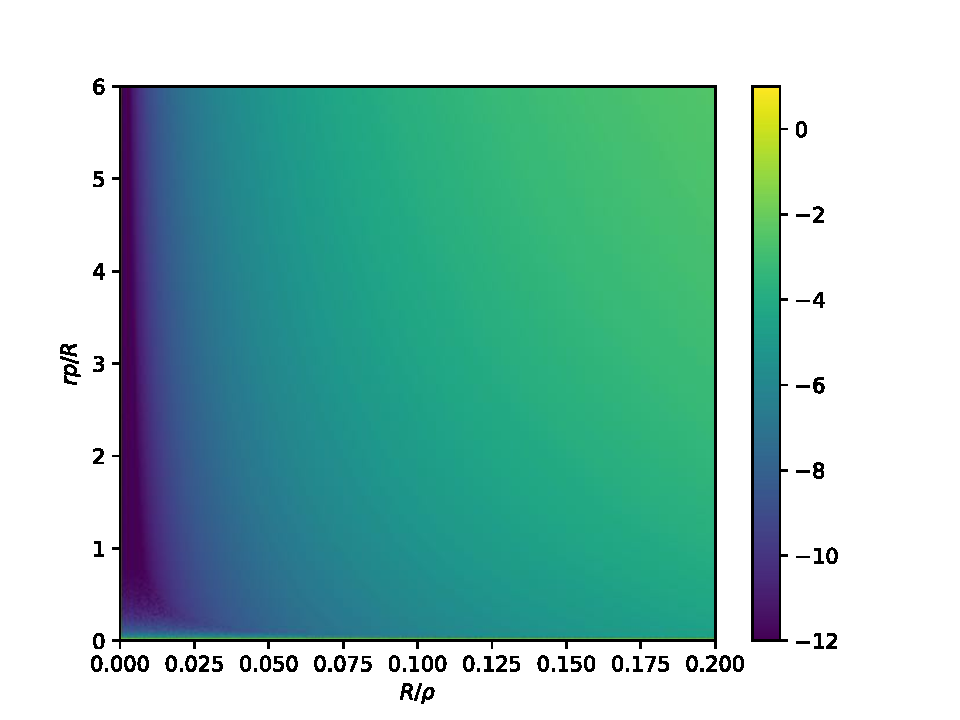
\includegraphics[width=\linewidth]{figs/extrapolation_error_plot_p6.pdf}
    \caption{\label{fig:extrap-err-p6}}
  \end{subfigure}
  \begin{subfigure}{.33\textwidth}
      \centering
      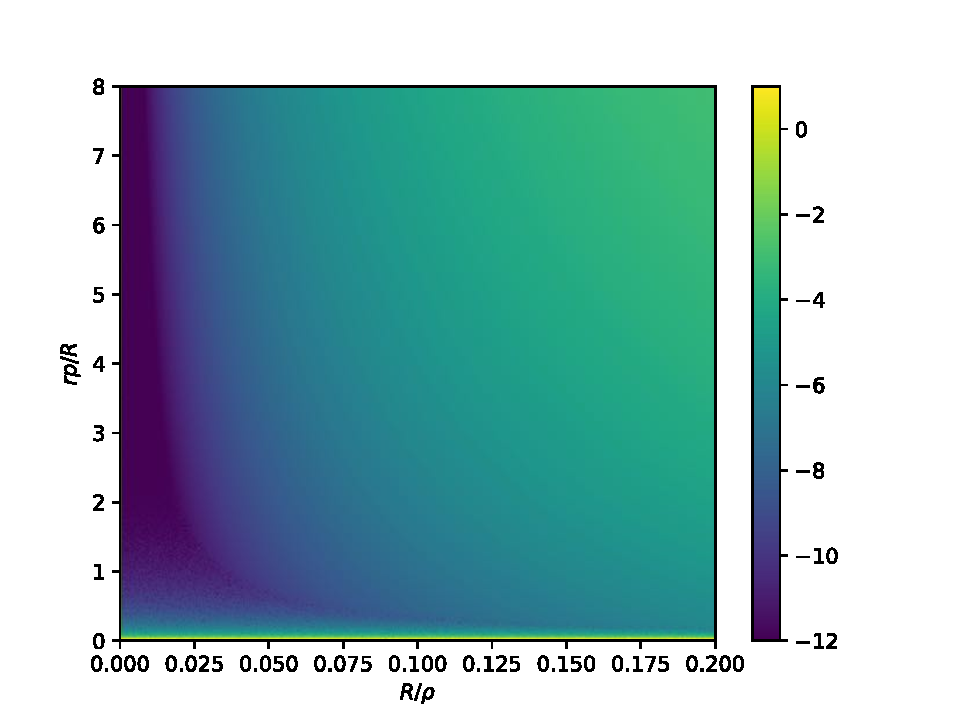
\includegraphics[width=\linewidth]{figs/extrapolation_error_plot_p8.pdf}
    \caption{\label{fig:extrap-err-p8}}
  \end{subfigure}%
    \begin{subfigure}{.33\textwidth}
      \centering
      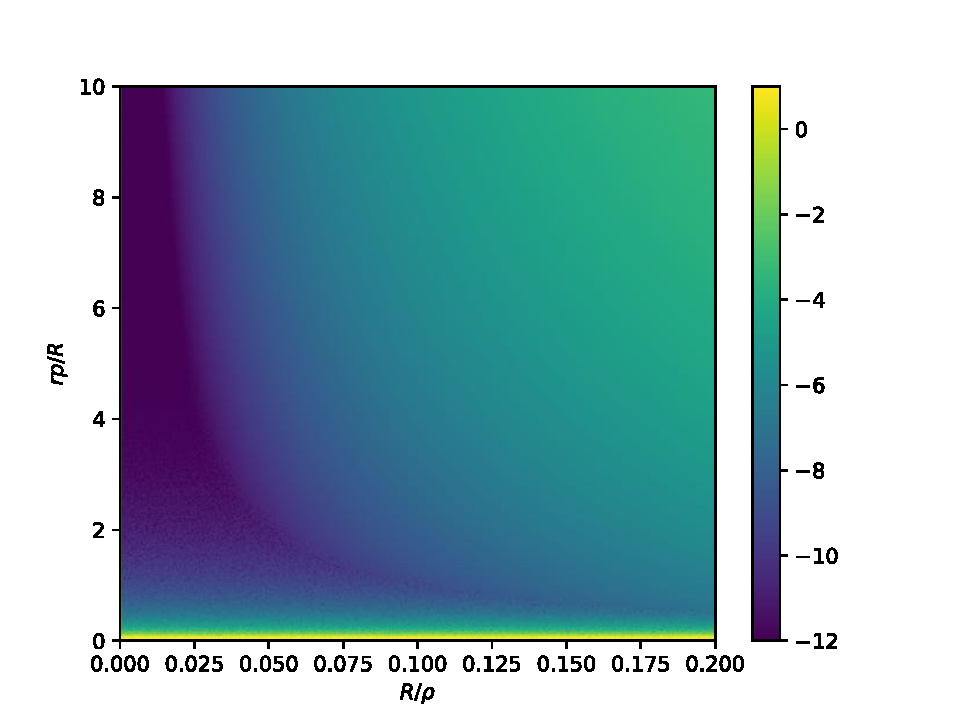
\includegraphics[width=\linewidth]{figs/extrapolation_error_plot_p10.pdf}
    \caption{\label{fig:extrap-err-p10}}
  \end{subfigure}
  \begin{subfigure}{.33\textwidth}
      \centering
      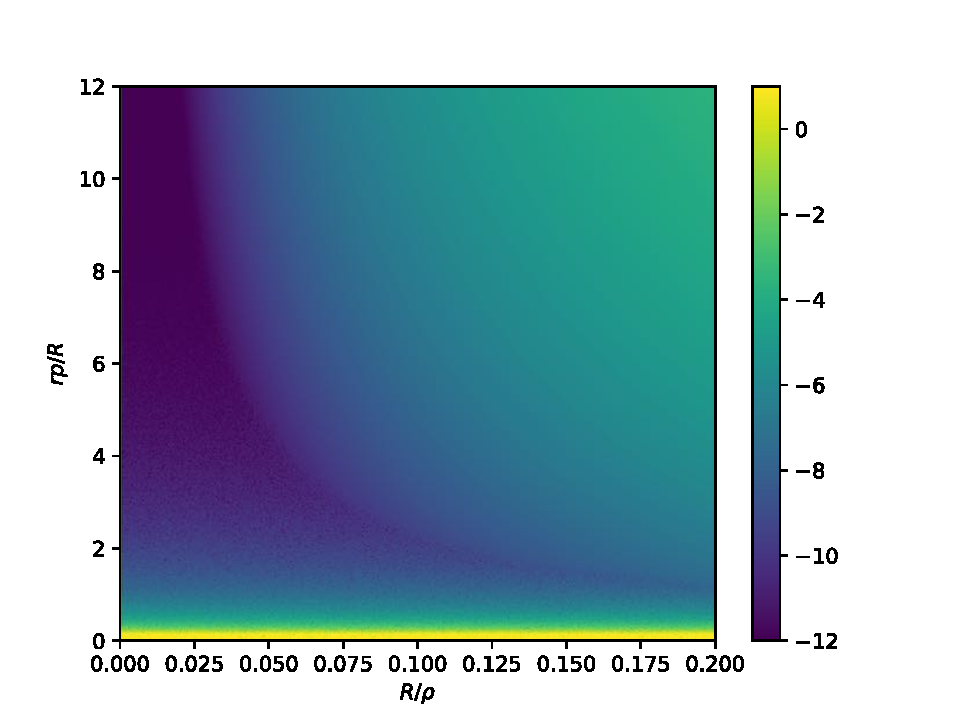
\includegraphics[width=\linewidth]{figs/extrapolation_error_plot_p12.pdf}
    \caption{\label{fig:extrap-err-p12}}
  \end{subfigure}%
  \begin{subfigure}{.33\textwidth}
      \centering
      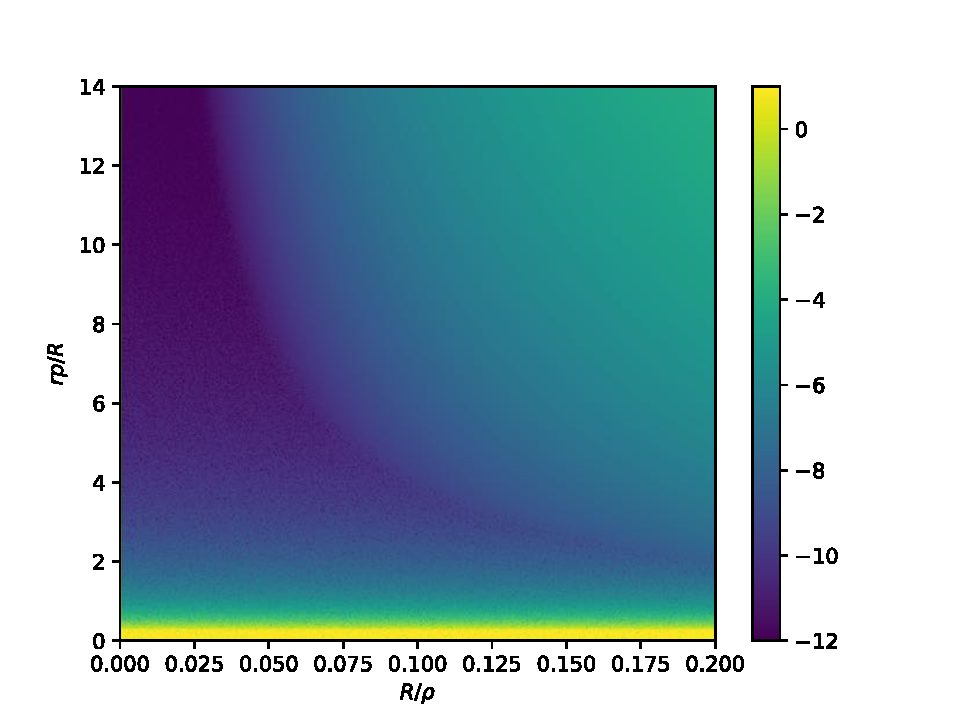
\includegraphics[width=\linewidth]{figs/extrapolation_error_plot_p14.pdf}
    \caption{\label{fig:extrap-err-p14}}
  \end{subfigure}%
  \mcaption{fig:extrap-experiment}{Empirical extrapolation error behavior}{We sweep over a range of $R$ and $r$ values to vary \Cref{fig:extrap-err-setup} and plot the log of the relative error in
    \Cref{fig:extrap-err-p6,fig:extrap-err-p8,fig:extrap-err-p10,fig:extrap-err-p12,fig:extrap-err-p14}, for values $p=6,8,10,12,14$, in increasing order, from (a) to (e).
In these figures, the $x$-axis is the extrapolation distance $R$ normalized by $\rho$ and the $y$-axis is the ratio $rp/R$.%: the total size of the approximation interval ($rp$) relative to the extrapolation distance $R$.
The top of the $y$-axis corresponds to $r=R$; $rp/R = 1$ corresponds to our choice of the parameter $a$.
Assuming that $\rho = O(L)$, $r/R = a/b$ and $R/\rho = b/\lambda$ for some constant $\lambda$.
}
\end{figure}
There are several important observations to make from these plots: 
\begin{itemize}
  \item Extrapolation error decreases as $R/\rho$ decreases, as expected.
  \item For a fixed value of $R/\rho$, the extrapolation error \textit{decreases} rapidly as $rp$ decreases, up to a certain value $r^*p$.
This is somewhat counterintuitive, since this means placing points closer together and extrapolating a further distance relative to $rp$.
For a fixed $p$ in exact arithmetic, letting the interpolation interval size tend to zero produces an order $p$ Taylor expansion of the solution $u$ centered at the interval's origin, which accounts for this phenomenon.

%\note[MJM]{Another interpretation of this result is from the perspective of Bernstein ellipses.
%Since $u$ is $C^\infty$ in a large neighborhood around the interval of interest, we can reason that the Bernstein parameter of the corresponding \oned approximation problem is growing as we decrease $rp$, thus increasing the convergence rate with respect to $R/\rho$.}

  \item Beyond $r^*p$, the extrapolation error \textit{increases}.
    The effects of finite precision eventually pollutes the convergence behavior described above. 
    Moreover, the spacing $r^*$ appears to be a function of $p$.
    For $p=6$, $r$ can be reduced to $1/p$ without any numerical issues, but
    by $p=14$, only $r>\frac{1}{2}$ is a safe choice for extrapolation.
\end{itemize}
We do not aim to rigorously analyze these phenomena in this work. 
We highlight them to provide empirical evidence that equispaced extrapolation is a reasonable, but not optimal, choice for our problem of singular/near-singular integration and to provide some intuition for our parameter choices.

The following simple result describes the behavior of the extrapolation error in \cref{eq:err-ext}.
\begin{theorem}
    Let $u(\vc(t))$ be the solution to \cref{eq:pde} given by \cref{eq:double_layer}, restricted to the line $\vc(t)$ in \threed intersecting $\vx$, let $\vc(t)$ be given by 
  \begin{equation}
    \vc(t) = \vsx - (R + tr)\vn(\vsx),
    \label{eq:check_point_param}
  \end{equation}
  where $\vsx$ is the closest point on $\Gammah$ to $\vx$, $R=bL_{\vsx}$, $r=aL_{\vsx}$, $\vn(\vsx)$ is the outward surface normal at $\vsx$, and let $|u^{(p)}(\vc(t))|$ be bounded above by $C_p$ on the interval $[-R, R+pr]$.
  Let $\mathfrak{P}(t)$ be the $p$-th order polynomial interpolant of $u(\vc(t))$ constructed from the check points $\vc_0, \hdots, \vc_p$, where $\vc_i = \vc(i)$. Then the extrapolation error associated with \qbkix behaves according to:
\begin{equation}
  |u(\vc(t_\vx)) - \mathfrak{P}(t_\vx)| \leq \frac{C_p}{(p+1)!}|R + rp|^p = \frac{C_p}{(p+1)!}|b+ap|^p\cdot | L|^p,
  \label{eq:extrap_err_init}
\end{equation}
where $t_\vx = \frac{\|\vx - \vsx\| - R}{r}$.
\label{thm:extrap_error}
\end{theorem}

\begin{proof}

    We know that for a smooth function $f$ and points $x_0, \hdots x_p$ in a \oned interval $I_0$, for some $\xi \in I_0$, the following relation holds for all $x \in I_0$:
\begin{equation}
    f(x) - \mathfrak{P}(x) = \frac{f^{(p)}(\xi)}{(p+1)!}\prod_{i=0}^p(x-x_i).
  \label{eq:exterp_err_init}
\end{equation}
Let $\mathfrak{P}$ be the $p$th order polynomial interpolating the points $x_0,\hdots x_p$.
In the \qbkix setup, since $R+rp$ is the distance of the furthest check point to $\vy$, we know that $x - x_i < R +rp$ for each $i$.
Since $f(t) = u(\vc(t))$ is harmonic, and therefore $C^\infty$, in $\Omega$, $|f^{(p)}(\xi)|$ can be uniformly bounded on $I_0$ by some constant $C_p$,
Noting that $R = bL$ and $r=aL$ yields our result.
\end{proof}

For fixed values of $a$ and $b$, as we let $L\to 0$, the extrapolation error is bounded by $O(L^p)$.
In practice, however, this means that we can choose $a$ and $b$ to minimize the constant factor $|b+ap|^p$ in \cref{thm:extrap_error}.
Since $p>1$, $a$ must be chosen to balance out the contribution of $p$, yet our extrapolation study shows that we can't simply set $a=0$.  
We therefore choose $a \leq 1/p$ for $p=6$ and 8, motivated by \cref{fig:extrap-err-p6,fig:extrap-err-p8}.
Moreover, since $b < 1$, we can choose $a \leq b/p$, which allows $a$ and $b$ to decay at the same rate.
%In exact arithmetic, $a$ controls how close the convergence order is to $p$.
%By holding $b$ fixed and letting $a\to 0$, we recover a $p$th order Taylor expansion of $u$ centered at $c_0$.
%Convergence to an approximate Taylor series is critical to the success of \qbkix and can be seen in \cref{fig:extrap-experiment}:
%we can improve extrapolation accuracy for a fixed value of $b$ by decreasing $a$, until numerical errors take over.
The advantage of choosing $a \leq b/p$ is that $b$ is a single parameter that controls the accuracy of \qbkix.
Since we have fixed the quadrature order $q=20$ to satisfy the assumption in \cref{sec:adaptive_upsampling}, a smaller value of $b$ will trigger more upsampling in \cref{alg:adaptive_upsampling}, keeping quadrature error fixed while reducing extrapolation error.

It is important to keep in mind that \cref{thm:extrap_error} only provides insight for moderate values of $p$; our conclusions are largely irrelevant for large $p$.
We use  $p = 6$ and $a = b/6$, leaving the construction of an optimal extrapolation extrapolation scheme to future work. 

\subsection{Geometry approximation error\label{sec:error_geom}}
Let $\theta$ be a scalar function defined on the surface of $\partial \Omega$ with $|\theta| \leq 1$ and let $\delta$ be a small real constant.
Suppose the boundary of the domain $\Omega$ is perturbed by $\delta$ along the normal field of $\partial\Omega$, scaled by $\theta$, to produce the perturbed domain $\Omega_\delta$ with boundary $\partial \Omega_\delta$.
More concretely, for $\vy \in \partial\Omega$ and $\vy_\delta\in \partial \Omega_\delta$, $\vy_\delta= \vy + \delta\theta\vn(\vy)$.
We can define the \textit{Eulerian shape derivative} of $u$ with respect to $\theta$, denoted $u_\theta$, at a point $\vx \in \Omega_\delta \cap \Omega$ as the rate of change in $u$ at $\vx$ as $\delta \rightarrow 0$.
This quantity is of interest to us because the solution to \cite[Equation 2]{morse2020robust} on $\Omega_\delta \cap \Omega$ can be written as $u + \delta u_\theta$, where $u$ is the solution to \cite[Equation 2]{morse2020robust} on $\Omega$.
Moreover, we can compute the shape derivative by solving a Laplace problem on the unperturbed domain \cite{pironneau1982optimal}:
\begin{equation}
\Delta u_\theta= 0\;\mbox{in $\Omega$, } u_\theta = -  \theta \frac{\partial u}{\partial n} \mbox{on $\partial\Omega$.}
\label{eq:shape-deriv}
\end{equation}  
where $u$ is the solution of the \cite[Equation 2]{morse2020robust} on $\Omega$.
For small $\delta$, this means that the error in the solution introduced by a boundary perturbation along the field $\theta$ can be estimated by  $\delta \sup_{\Omega} \| u_\theta \|$.
Assuming the boundary is smooth and the gradient of the solution $u$ is bounded, then
\begin{equation}
\| u_\theta \| \leq C_g \sup_{\partial\Omega} \left| \theta  \frac{\partial u}{\partial n} \right| \leq
C_g \sup_{\partial\Omega} \left| \frac{\partial u}{\partial n}\right|
\label{eq:shape-deriv-bound}
\end{equation}
for some real constant $C_g$.
The right-hand side of \cref{eq:shape-deriv-bound} yields a constant $C_g^\prime$, such that if $\err{g} <  \zeta\etrg/C_g^\prime$ for some $\zeta < 1$,  the change in the solution is less than $\etrg$ for a sufficiently small $\err{g}$.
%\note[DZ]{Need to find (again) a reference saying this, as this is not true for general boundaries}
The constant depends implicitly on the surface geometry: for example, if an area element of $\partial\Omega$ is close to a sharp, concave corner, then  $\frac{\partial u}{\partial n}$ can be arbitrarily large. 


\subsection{Limitations \label{sec:limitations}}
Our error discussion reveals several limitations of our method. 
The first and most apparent shortcoming is that extrapolation instability fundamentally limits convergence order. 
However, for reasonable orders of convergence, up to 14, we have discussed an empirical scheme to choose parameters to maximize the available convergence behavior.
Moreover, low-order surface geometries used in engineering applications will likely limit the convergence rate before it is limited by the extrapolation order, making this a non-issue in practical scenarios.

Another downside of the chosen extrapolation approach is lack of direct extension of \qbkix to oscillatory problems like the Helmholtz equation.
Due to the limitation on the values of $p$, we can't guarantee the ability to resolve high-frequency oscillations in the solution.
A new extrapolation procedure is required to do so robustly without compromising efficiency.

In \cite{wala20193d}, the authors demonstrate a relationship between the truncation error of a \qbx expansion and the local curvature of $\Gammah$. 
Our scheme also is susceptible to this form of error and we do not address nor analyze this in this work.
This is a subtle problem that requires a detailed analysis of the surface geometry with respect to the chosen extrapolation scheme.
%We leave this to a future work that produces an optimal extrapolation approach in the boundary integral context.
Another  limitation is the lack of an accurate error estimate to serve as an upsampling criteria in place of the criteria in \cref{sec:adaptive_upsampling}, such as \cite{klinteberg2019accurate}. 
Extending \cite{klinteberg2019accurate} to \threed surfaces is non-trivial and whether the size of $\Pfine$ would be reduced enough to outweigh the added cost of the additional Newton iterations required by their scheme remains to be seen.

Finally, for certain accuracy targets and geometries, the algorithm above may lead to an impractically high number of patches in $\Pcoarse$ and $\Pfine$. 
Geometries with nearly-touching non-local regions, as shown in \cref{fig:torii}, will see large amounts of refinement.
If the nearly-touching embeddings $\gamma_r$ are close enough, i.e., less than $10^{-10}$ apart, there is little hope of an accurate solution with a fixed computational budget.
We allow the user to enforce a minimal patch size $L_\lbl{min}$, limiting the time and memory consumption at the expense of not reaching the requested target accuracy. 
